% Created 2023-03-02 Thu 11:55
% Intended LaTeX compiler: pdflatex
\documentclass[11pt,english,a4paper]{article}
\usepackage[utf8]{inputenc}
\usepackage[T1]{fontenc}
\usepackage{graphicx}
\usepackage{longtable}
\usepackage{wrapfig}
\usepackage{rotating}
\usepackage[normalem]{ulem}
\usepackage{amsmath}
\usepackage{amssymb}
\usepackage{capt-of}
\usepackage{hyperref}
\usepackage[left=1in,right=1in,top=0.75in,bottom=0.75in]{geometry}
\usepackage[capitalize,noabbrev]{cleveref}
\author{Ragnar Groot Koerkamp}
\date{\textit{<2022-12-12 Mon>}}
\title{Doctoral plan\\\medskip
\large Near-linear exact pairwise alignment}
\hypersetup{
 pdfauthor={Ragnar Groot Koerkamp},
 pdftitle={Doctoral plan},
 pdfkeywords={},
 pdfsubject={},
 pdfcreator={Emacs 28.2.50 (Org mode 9.6)}, 
 pdflang={English}}
\usepackage[style=authoryear]{biblatex}
\addbibresource{/home/philae/git/eth/research/references.bib}
\begin{document}

\renewcommand{\ref}{\cref}
\begin{titlepage}
\center % Center everything on the page
\textsc{\LARGE Ph.D. Doctoral plan}\\[1.5cm]
\setlength{\baselineskip}{25pt}
{ \huge \bfseries Near-linear exact pairwise alignment}

\vspace{1.5cm}

\begin{minipage}{0.35\textwidth}
\begin{flushleft} \large
\emph{Ph.D. Candidate:}\\
Ragnar \textsc{Groot Koerkamp} \\
\emph{21-961-677}
\end{flushleft}
\end{minipage}
~
\begin{minipage}{0.34\textwidth}
\begin{center} \large
\emph{Supervisor:} \\
Prof. Dr. Gunnar  \textsc{R\"{a}tsch} \\
\phantom{}
\end{center}
\end{minipage}
~
\begin{minipage}{0.25\textwidth}
\begin{flushright} \large
\emph{Second advisor:} \\
Dr. Erik  \textsc{Garrison} \\
\phantom{}
\end{flushright}
\end{minipage}\\[4cm]
\textsc{ETH Z\"{u}rich} \\
Department of Computer Science\\
Biomedical Informatics Group\\
\emph{Started:} May 2022\\
\vfill
\end{titlepage}

\section{Research Proposal: Near-linear exact pairwise alignment}
\label{sec:orge4142b1}

\subsection{Abstract}
\label{sec:org5ab1fef}
\emph{Pairwise alignment} and \emph{edit distance} specifically is a problem that was
first stated around 1968 \autocite{nw,vintsyuk68}. It involves finding the minimal
number of edits (substitutions, insertions, deletions) to transform one string/sequence
into another.
For sequences of length \(n\), the original algorithm takes \(O(n^2)\) quadratic
time \autocite{sellers}.
In 1983, this was improved to \(O(ns)\) for sequences with low edit distance \(s\)
using Band-Doubling. At the same time, a further improvement to
\(O(n+s^2)\) expected runtime was presented using the diagonal-transition method \autocite{ukkonen83,ukkonen85,myers86}.

Since then, the focus has shifted away from improving the algorithmic complexity
and towards more efficient implementations of the algorithms, using e.g.
bit-packing, delta-encoding, and SIMD
\autocite{myers99,edlib,difference-recurrence-relations}.

Meanwhile, the edit distance problem was also generalized to \emph{affine costs}
\autocite{gotoh}, which is a biologically more relevant distance metric when
computing the \emph{distance} between DNA sequences.
It appears that the \(O(n+s^2)\) diagonal transition algorithm was
mostly forgotten, until recently it was generalized to also handle affine costs
and implemented efficiently in WFA and BiWFA \autocite{wfa,biwfa}.
This has sparked new interest in pairwise alignment from the field of
computational biology, and makes it possible to align significantly longer
sequences provided they have a sufficiently low error rate.

In this PhD, I first want to thoroughly understand existing
algorithms, their implementations, and their performance characteristics on
various types of data.
Then, the goal is to design efficient near-linear exact global pairwise alignment
algorithms by building on the A* framework first introduced in Astarix
\autocite{astarix-1,astarix-2} and combining this with the implementation efficiency of
WFA and Edlib.

A*PA has already shown over \(200\times\) speedup over these tools on \(10^7\) bp
long sequences with uniform errors. However, on alignments with long indels or
too high error rate A*PA is currently slower because it needs \(\sim 100\times\)
more time per visited state than SIMD-based approaches. Future iterations are
expected to decrease this gap and lead to an aligner that outperforms
state-of-the-art methods by at least \(10\times\) on various types of data.

\subsection{Introduction and current state of research in the field}
\label{sec:orgecc00e2}

Computing \emph{edit distance} is a classic problem in computer science and
Needleman-Wunsch \autocite{nw,sellers} is one of the
prime examples of a dynamic programming (DP) algorithm.
This problem naturally arises in bioinformatics, where it corresponds to finding
the number of biological mutations between two DNA sequences. In this setting,
the problem is usually referred to as \emph{pairwise alignment}, where not only the
distance but also the exact mutations need to be found. As such,
biological applications have always been a motivation to develop faster
algorithms to solve this problem:
\begin{itemize}
\item the original \(O(n^2)\) Needleman-Wunsch algorithm \autocite{nw,sellers} that is
quadratic in the sequence length \(n\);
\item the \(O(ns)\) Dijkstra's algorithm that is faster when the edit distance \(s\) is small;
\item the \(O(ns)\) band-doubling algorithm \autocite{ukkonen85} that allows a much more
efficient implementation;
\item the even faster \(O(n+s^2)\) expected runtime diagonal-transition algorithm \autocite{ukkonen85,myers86}.
\end{itemize}
The biological application has motivated a generalization of the edit distance
problem to \emph{affine gap-costs} \autocites{waterman}[][]{gotoh}[][]{wfa}, where the cost of
a gap of length \(k\) is an \emph{affine} (as opposed to \emph{linear}) function of \(k\),
i.e. \(open + k\cdot extend\).  This better models the relative probabilities of
biological mutations.

In recent years DNA sequencing has advanced rapidly and increasingly
longer DNA sequences are being sequenced and analysed. Now that so called
\emph{long reads} are reaching lengths well over \(10k\) base pairs, even up to \(100k\)
bp for some sequencing techniques, the classical quadratic algorithms do not
suffice anymore. This has caused a few lines of research:
\begin{enumerate}
\item The Needleman-Wunsch and band-doubling algorithms have been improved using
\emph{bit-packing} and \emph{delta encoding}, where multiple DP states are stored and
computed in a single computer word
\autocite{myers99,difference-recurrence-relations}, as implemented by Edlib \autocite{edlib}.
\item Advances in hardware have further enabled more efficient
implementations of the existing algorithms using better data layouts and
SIMD, as used by Parasail \autocite{parasail}, WFA \autocite{wfa}, WFA-GPU
\autocite{wfa-gpu}, and block aligner \autocite{block-aligner}.
\item Many inexact (heuristic) methods have been proposed to speed up alignment
significantly, at the cost of not having a guarantee that the returned
alignment is optimal.
\end{enumerate}

Despite these advances, the fastest exact pairwise alignment algorithms still
scale quadratically with sequence length on data with a constant error rate.

My research starts with the recent introduction of A* to sequence-to-graph
alignment \autocites{astarix-2}[][]{astarix-1}. We applied similar ideas to pairwise
alignment, and it turns out that A* with some additional techniques is able to
lower the runtime complexity from quadratic to near-linear on sequences with a
low uniform error rate \autocite{astarpa}.

\subsection{Goals of the thesis}
\label{sec:orgc25a27e}
Here I list the main goals of this thesis. They are discussed in more detail in
\ref{sec:orgfbb2d6a}.

The main goals of this thesis fall into two categories:
\begin{description}
\item[{Comparing existing methods}] Understand, analyse, and compare existing
alignment algorithms, implementation techniques, and tools.
\begin{description}
\item[{Theory}] \emph{Conceptually understand existing algorithms and techniques.}

First, I want to obtain a thorough understanding of all existing algorithms and
implementations on a conceptual level.
As listed in the introduction, there are multiple different existing algorithms
(DP, Dijkstra, band-doubling, diagonal-transition), and each come with their own
possible optimizations (SIMD, difference-recurrences, bit-packing).
\item[{Practice}] \emph{Benchmark existing tools/implementations on various types of data.}

Secondly, a thorough benchmark comparing these algorithms and implementations
does currently not exist, but is needed to understand the trade-offs between
techniques and alignment parameters and improve on the state-of-the-art.
\item[{Visualization}] \emph{Visualize new and existing algorithms.}

Visualizations make algorithms much easier to understand, explain, and teach, and
can even help with comparing performance of difference methods and debugging.
\end{description}
\end{description}


\begin{description}
\item[{New methods}] Develop A*PA, a new near-linear algorithm and implementation for exact
pairwise alignment that is at least \(10\times\) faster than other methods on most types
of input data.
\begin{description}
\item[{A*PA v1: initial version}] Apply the seed heuristic of Astarix
\autocite{astarix-2} to exact global pairwise alignment and extend it with
chaining, gap-costs, pruning, and diagonal-transition.
\item[{A*PA v2: efficient implementation}] Speed up the implementation using
SIMD. This merges ideas from block aligner \autocite{block-aligner} and
\emph{global} band-doubling \autocite{ukkonen85} into \emph{local} column- or block-based doubling.
\item[{Scope: affine costs}] Generalize the scope to affine-cost alignments.
This will require new ways to efficiently compute the heuristic due to the
more complex cost-model.
\item[{Scope: ends-free alignment and mapping}] Support semi-global and extension
alignment, and support efficiently aligning multiple reads against a single
reference.
\item[{Further extensions}] A non-admissible heuristic could lead to faster
approximate algorithms. Alternatively, a guessed inexact alignment could
speed up finding a correct alignment or proving it is correct.
\end{description}
\end{description}

Lastly, there are many other interesting problems to which our A*-based results
could be extended. In genome assembly, the task is to  such as assemble DNA for
a large set of reads, and best-overlapping reads may be found using A*.
In RNA folding, the task is to optimally fold an RNA sequence onto itself. This
is another classic DP problem, and it may benefit from A* by penalising local
folds that have a bad score.  Lastly, it may be possible to extend the pruning
introduced by A*PA to real-world route planning.  All these problems fall in a
category of \textbf{open ended research}, if time permits.

\subsubsection{Impact}
\label{sec:org6eb65d4}
Many types of pairwise alignment are used in computational biology. Many
inexact (heuristic) approaches have been developed to keep alignments
sufficiently fast given the increasing size of sequences that are being aligned and
the increasing amount of biological data available. A faster exact algorithm
reduces the need to fall back to inexact methods, and reduces the need to accept
the possibility of suboptimal alignments.

To increase the scope of practical applications, we will extend support to
semi-global and affine cost alignments.

\subsection{Progress to date}
\label{sec:org24b2838}
\textbf{Theory:} Reading the existing literature has lead to multiple blogs posts collecting
information and ideas. This includes
\href{https://curiouscoding.nl/posts/pairwise-alignment/}{a systematic overview} (\href{https://curiouscoding.nl/posts/pairwise-alignment}{curiouscoding.nl/posts/pairwise-alignment}) of over 20 algorithms and papers on pairwise alignment,
including a table comparing them and illustrations of the parameters and algorithms.

The literature also sparked multiple ideas and smaller observations regarding WFA:
\begin{itemize}
\item I \href{https://github.com/smarco/WFA2-lib/issues/8}{suggested} using divide and conquer \autocite{hirschberg75} for WFA, which
turned out to be already in development as BiWFA, and found a \href{https://github.com/smarco/BiWFA-paper/issues/8}{related bug} in
the preprint \autocite{biwfa}.
\item \href{https://curiouscoding.nl/posts/linear-memory-wfa/}{Ideas} to reduce the memory usage by WFA and other algorithms needed for tracebacks.
In essence, the tree of paths to the last front is very sparse, and typically
requires much less memory to store than the full set of wavefronts.
\item Some further notes regarding \href{https://curiouscoding.nl/posts/wfa-variations/}{variants of the recursion}, \href{https://curiouscoding.nl/posts/diamond-optimization/}{reducing the number of
visited states}, and \href{https://curiouscoding.nl/posts/alignment-scores-transform/}{an improved way to handle match bonus}.
\end{itemize}

\textbf{Benchmarking:} Together with Daniel Liu, I developed PaBench
(\href{https://github.com/pairwise-alignment/pa-bench}{github.com/pairwise-alignment/pa-bench}), a tool to help benchmarking pairwise
aligners. It provides a uniform interface to many existing aligners as part of
the \emph{runner} binary, and contains an \emph{orchestrator} that can run a large number
of alignment jobs as specified via a YAML configuration file. Possible
configuration options are selecting the datasets to run on (files, directories,
generated data, or downloaded data), which cost-model to use, and which aligners
to run and their parameters. This makes it very quick and easy to generate plots
such as \ref{gap_open_scaling}, showing that when aligning unrelated/independent
sequences Edlib for unit-cost alignments is around \(30\times\) faster than any
affine alignment that includes a gap-open cost.

\begin{figure}[t]
\centering
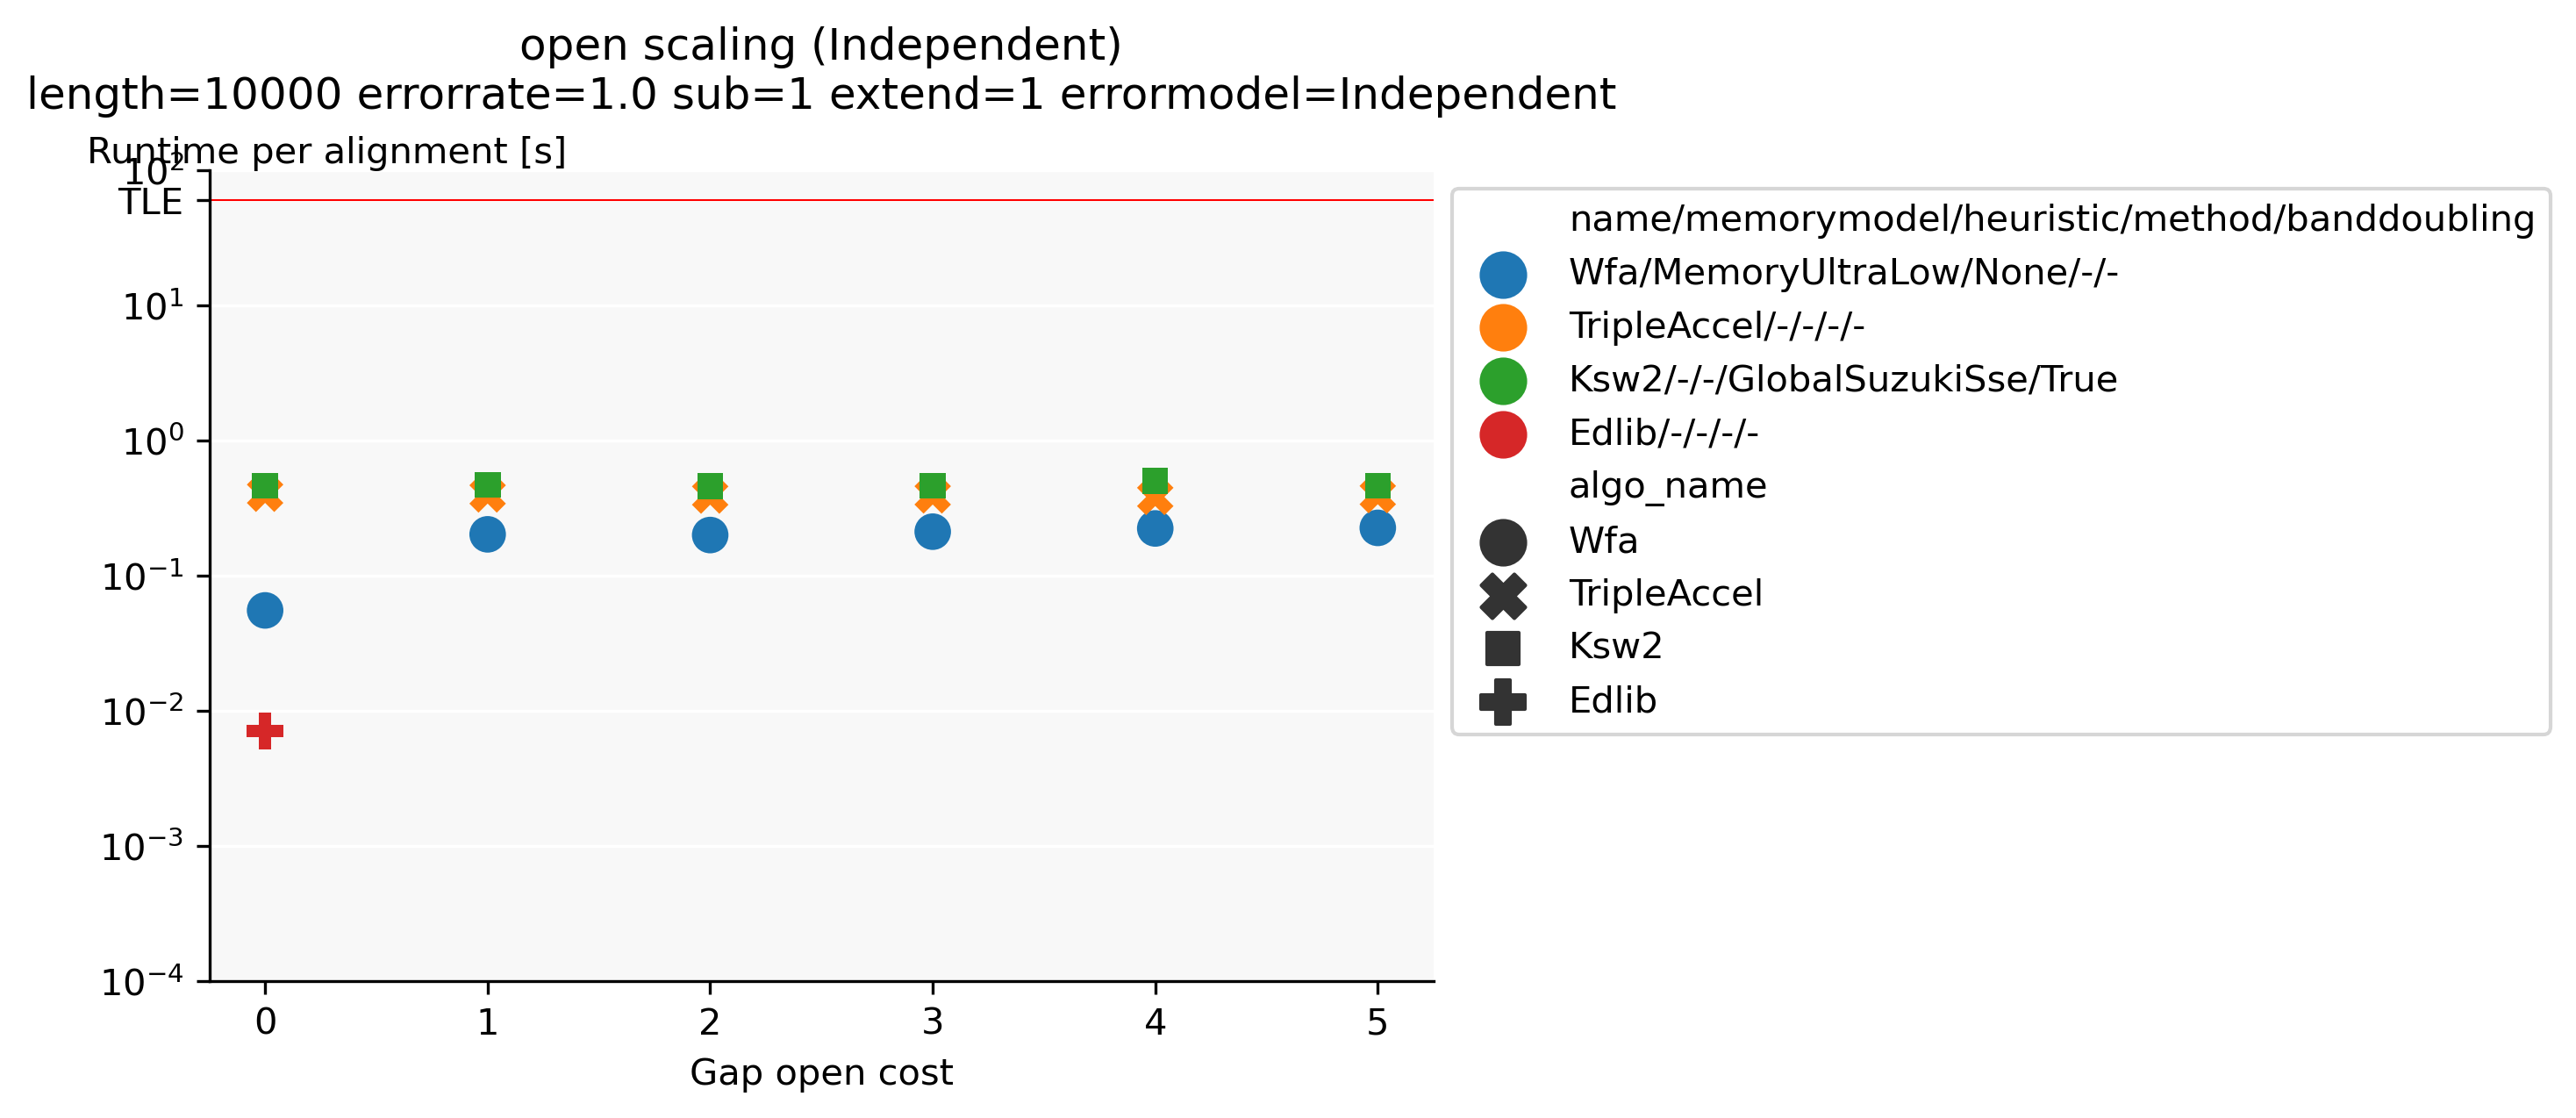
\includegraphics[width=.9\linewidth]{./gap_open_scaling_Independent.png}
\caption{\label{gap_open_scaling}Runtime comparison between different aligners when aligning two complete independent random sequences, for various gap-open costs. The substitution and gap-extend cost are fixed to 1. Edlib only supports a gap-open cost of \(0\).}
\end{figure}

\textbf{Visualization:}
I wrote a visualizer to show the inner workings of A*PA and to help with
debugging. The existing Needleman-Wunsch, band-doubling, and diagonal-transition
algorithms were re-implemented to understand their inner workings and to make
for easy visual comparisons, as shown in \ref{vis}.

\begin{figure}[t]
\centering
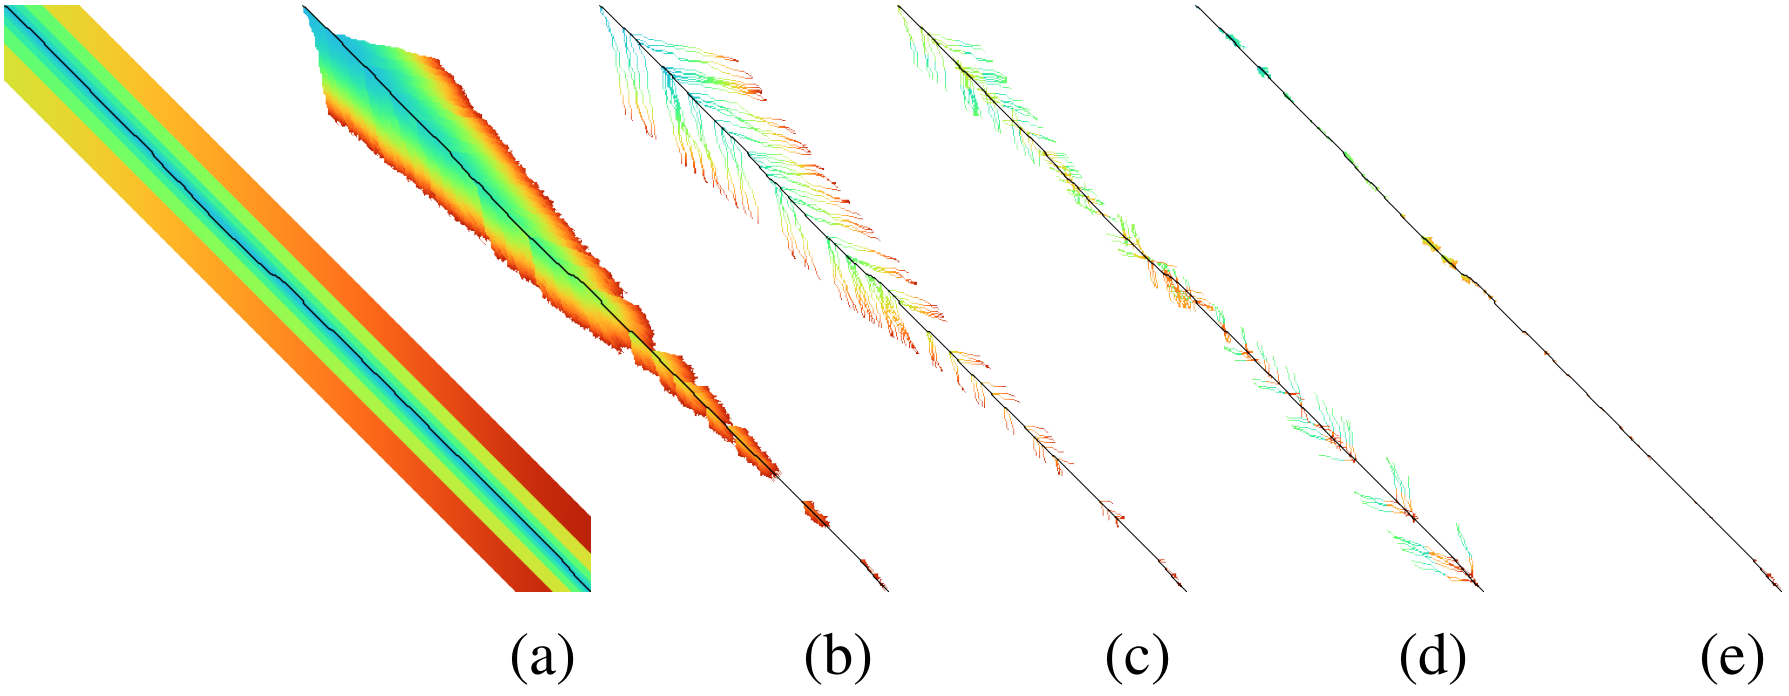
\includegraphics[width=.9\linewidth]{./vis.png}
\caption{\label{vis}Visualizations of (a) band-doubling (Edlib), (b) Dijkstra, (c) diagonal-transiton (WFA), (d) diagonal-transition with divide-and-conquer (BiWFA), and (e) A*PA.}
\end{figure}

\textbf{A*PA v1:}
The first version of \href{https://github.com/RagnarGrootKoerkamp/astar-pairwise-aligner}{A*PA} has been implemented at
\href{https://github.com/RagnarGrootKoerkamp/astar-pairwise-aligner}{github.com/RagnarGrootKoerkamp/astar-pairwise-aligner} and is evaluated
in a preprint \autocite{astarpa}.
The current codebase implements the following techniques:
\begin{itemize}
\item \emph{seed heuristic} \autocite{astarix-2}, the basis for the A* search,
\item \emph{match-chaining} to handle multiple matches,
\item \emph{gap-costs}, to account for gaps between consecutive matches (not yet in preprint),
\item \emph{inexact matches}, to handle larger error rates,
\item \emph{match-pruning}, penalizing searching states that lag behind the tip of the search,
\item \emph{diagonal-transition}, speeding up the search by skipping over states that are
not \emph{farthest-reaching} (not yet in preprint).
\end{itemize}

Together this has already shown promising results with linear runtime scaling
on sequences with a low uniform error rate, resulting in up to \(250\times\) speedup over
other aligners for sequences of length \(10^7\) bp (\ref{scaling}).

\begin{figure}[h]
\centering
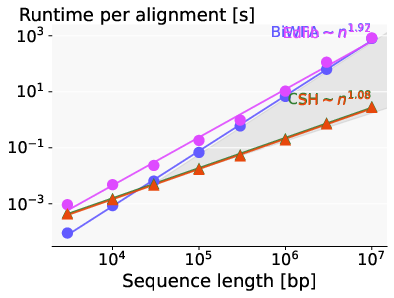
\includegraphics[width=0.5\textwidth]{scaling.png}
\caption{\label{scaling}Runtime scaling of A*PA with seed heuristic (SH) and chaining seed heuristic (CSH) on random sequence-pairs of given length with constant uniform error rate \(5\%\).}
\end{figure}

\subsection{Detailed work plan}
\label{sec:orgfbb2d6a}
The work is split over the following \(9\) concrete projects, ordered by
estimated order of completion.

\subsubsection{WP1: A*PA v1: initial version}
\label{sec:org7faa189}
A*PA \autocite{astarpa} introduces the seed heuristic of \textcite{astarix-2}
(\ref{astarpa} a) that provides a lower bound on the edit distance between (the
suffixes of) two sequences by counting the number of \emph{seeds} without \emph{matches}:
for each seed (disjoint substring of sequence \(A\)) that does not occur in
sequence \(B\), there must be at least \(1\) edit to turn \(A\) into \(B\).

\begin{figure}[h]
\centering
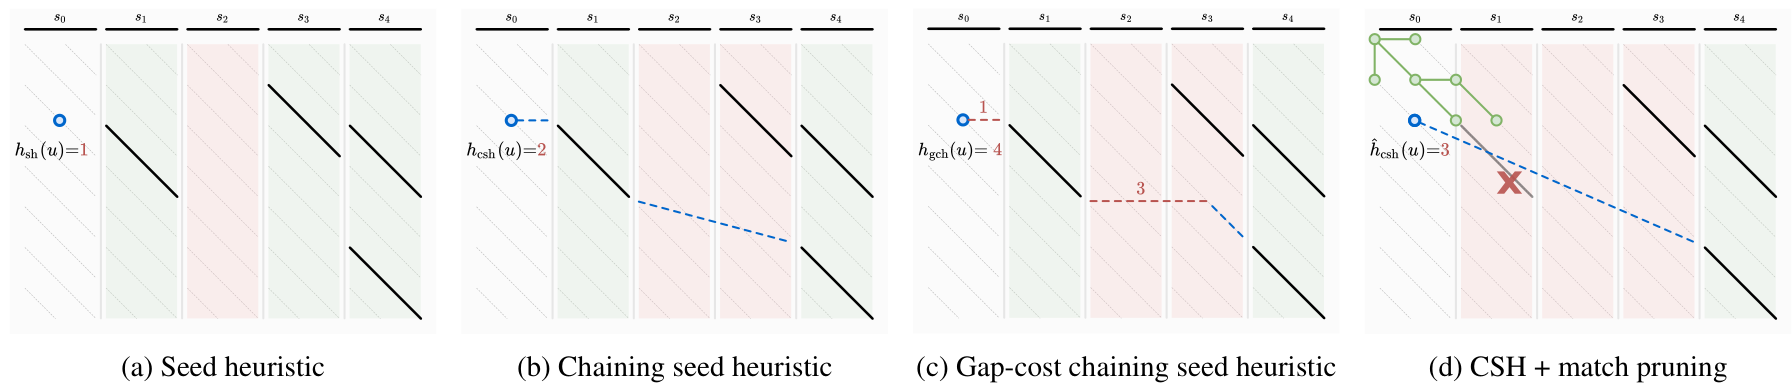
\includegraphics[width=.9\linewidth]{astarpa.png}
\caption{\label{astarpa}The different heuristics and techniques introduced by A*PA.}
\end{figure}

A*PA extends this in a few ways. See the preprint for more details.
\begin{itemize}
\item First, it introduces \emph{inexact matches}, where a \emph{match} is considered to be
any substring of \(B\) that less than distance \(r\) away from the seed. This
allows the A* to efficiently handle larger error rates.
\item The \emph{chaining seed-heuristic} (b) requires seed-matches to be in the same
order in \(B\) as in \(A\). This way, spurious matches have less negative effects
on the value of the heuristic.
\item The \emph{gap-cost chaining seed heuristic} (c) additionally penalizes the
cost that must be made for indels between matches that are on different diagonals.
\item \emph{Pruning} (d) is an additional technique that penalizes searching behind the \emph{tip}
of the search. As soon as the start of a match is expanded, the match is not
needed anymore and can be removed. This makes the heuristic inadmissible, but
we prove that A* is still guaranteed to find an optimal path.
\item Lastly, we use an optimization similar to diagonal-transition so that only
\emph{farthest-reaching states} are expanded by the A*.
\end{itemize}

This results in near-linear scaling (\ref{scaling}) when aligning long sequences with low constant uniform error
rate, leading to \(250\times\) speedup over state-of-the-art aligners WFA and Edlib.

\textbf{Status:} This work package is almost done and will be submitted to
 BioInformatics in the first week of April 2023.

\subsubsection{WP2: Visualizing aligners}
\label{sec:org1294108}
There are many existing algorithms for pairwise alignment, many of which are
more than 30 years old. Some papers \autocite{ukkonen85,block-aligner} contain
manual figures depicting the working of an algorithm, but other papers do not
\autocite{edlib,wfa}. This limits the quick intuitive understanding of such
algorithms. Since pairwise alignment happens on a 2D DP grid it allows for
easy-to-understand visualizations where fewer coloured pixels (visited states)
usually imply faster algorithms. This not only makes it easier to teach these algorithms
to students but also helps with debugging and improving performance: an
image makes it easy to understand the structure of an alignment and to spot
bottlenecks in algorithms.

\textbf{Status:} This work package is done and used for e.g. \ref{vis}. Visualizations will
be added as new methods are developed.

\subsubsection{WP3: Benchmarking aligners}
\label{sec:org18ba3e7}
A good understanding of the performance trade-offs of existing aligners is
needed in order to improve on them.
While all recent papers presenting aligners
contain benchmarks comparing them in some specific setting,
there is no thorough recent overview of tools that compares runtime and accuracy on all of the
following properties:
\begin{itemize}
\item input type: either random or human,
\item error type: uniform or long indels,
\item error rate,
\item sequence length,
\item cost model: unit costs, linear costs, or affine costs,
\item algorithm parameters,
\item heuristics for approximate results.
\end{itemize}

For example, Edlib \autocite{edlib} lacks a comparison on non-random data, whereas
the \(O(n+s^2)\) expected runtime WFA \autocite{wfa} is only benchmarked against
\(O(n^2)\) algorithms for exact affine-cost alignment, and not against \(O(ns)\)
algorithms. In fact, no efficient \(O(ns)\) affine-cost aligner had been
implemented until Daniel Liu and I recently improved KSW2. Furthermore,
unit-cost alignment and affine-cost alignment are usually considered as distinct
problems, and no comparison has been made about the performance penalty of
switching from the simpler unit-cost alignments to more advanced affine costs.

\textbf{Status:} The implementation part of this work package is done and used to
benchmark A*PA and make figure \ref{gap_open_scaling}. A thorough comparison of tools
is still pending.

\subsubsection{WP4: Theory review}
\label{sec:org699015d}
There is no review paper of exact global alignment methods.
\textcite{navarro01} seems to be the most relevant,
but focuses on semi-global alignment (\emph{approximate string matching}) instead.
Either way, there has been a lot of progress since
that paper was published:
\begin{itemize}
\item computer hardware has improved, allowing for SIMD based methods,
\item new recurrence relations have been found \autocite{difference-recurrence-relations},
\item new algorithms have been implemented (KSW2, WFA, Edlib, block aligner).
\end{itemize}
Thus, the time is right for a new review summarizing both the
various algorithms and implementation strategies used in modern pairwise
aligners.
This would also include a discussion of implicit previous uses of A* and
heuristics, and how changing to an equivalent cost model can have an effect equivalent
to using a heuristic.

\textbf{Status:} Most of the literature has been summarized in a blog post as part of
the background research for A*PA. A dedicated paper has not yet been started.

\subsubsection{WP5: A*PA v2: efficient implementation}
\label{sec:org819e8ca}
The biggest bottleneck of the current A*-based implementation is the need to
store information for each visited state in a hashmap and priority queue.
Each visited state has to go through the following process:
\begin{enumerate}
\item Check if it was already expanded before in the hashmap.
\item Evaluate the heuristic.
\item Push it on the priority queue.
\item Pop it from the priority queue.
\item Evaluate the heuristic again.
\item Update the hashmap.
\end{enumerate}

It turns out that this is up to \(100\) times slower per state than Edlib, which
only stores \(2\) bits per state and can compute \(32\) states at a time using
bit-packing.

To speed up A*PA, it will be needed to compute multiple states at once so that
bit-packing or SIMD can be used.
One way this could work is \emph{local doubling}.
Similar to the band-doubling technique introduced by Ukkonen and used by Edlib
\autocite{ukkonen85,edlib}, it is possible to efficiently process states
column-by-column and revisit previous columns when it turns out more states need
to be computed.

It works by choosing some threshold \(f\) and computing all states \(u\) with \(f(u)
:= g(u) + h(u) \leq f\) from left to right (column by column). When a column has
no states with \(f(u) \leq f\), this means that the distance between the two
strings is more than \(f\), and the threshold must grow. Ignoring pruning, this would
work roughly as follows:
\begin{enumerate}
\item For each column \(i\) store the last value of \(f_i\), which starts at the value
of the heuristic in \(0\), and
store the last \emph{increment} per column \(\Delta_i\) which starts at \(1\).
\item For increasing \(i\) starting at \(0\), find the range of
column \(i\) with \(f(u) \leq f_i\) and compute the distance to these cells.
\item As soon as the range is empty for some column, \emph{backtrack} and double the band for
previous columns:
\begin{enumerate}
\item For \(j\) going down from \(i-1\), add \(\Delta_{j}\) to \(f_{j}\) and double \(\Delta_{j}\).
\item When \(f_{j-1} \geq f_{j}\), stop decreasing \(j\) further.
\item Now continue with step 2, increasing \(i\) starting at \(i=j\).
\end{enumerate}
\end{enumerate}

The result of this process can be seen in \ref{local-doubling}. Note that this does
not yet account for pruning, where some difficulties remain to be solved. In
particular, the algorithm relies on the fact that doubling \(\Delta_i\) roughly
doubles the computed band. Since pruning changes the value of the heuristic,
this is not true anymore, and the band often grows only slightly. This breaks
the exponential doubling and hence causes unnecessarily large runtimes. A
possible way to improve this could be enforce at least a doubling of
the computed band.

In the current implementation, computing the heuristic at the top and bottom of
each band (to find the range where \(f(u) \leq f_i\)) and storing the computed
values for each column require a lot of overhead. Using \emph{blocks of
columns} as in block aligner \autocite{block-aligner} could significantly reduce
this, since then the bookkeeping would only be needed once every \(8\) to \(32\) columns.

\begin{figure}[htbp]
\centering
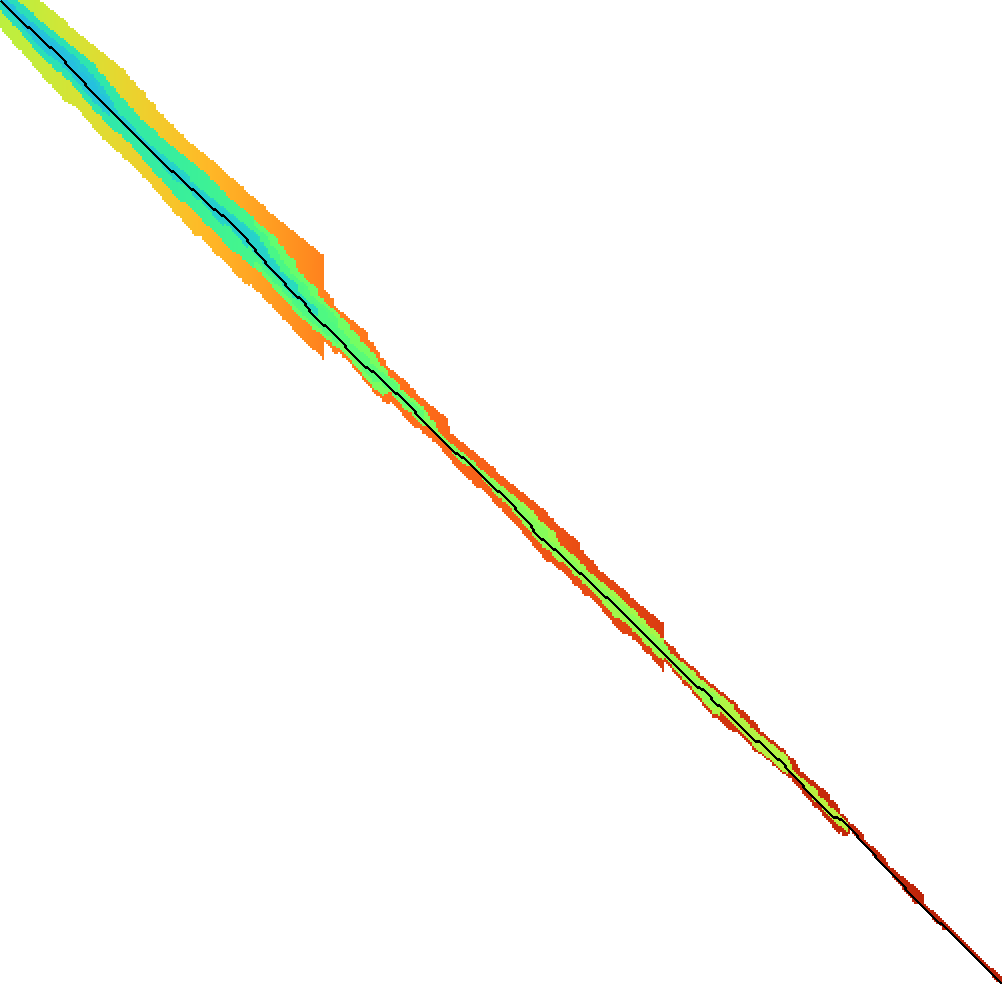
\includegraphics[width=0.4\textwidth]{local-doubling.png}
\caption{\label{local-doubling}Expanded states with local doubling.}
\end{figure}

It is still an open problem to find an efficient doubling strategy when pruning
is enabled, but even without that or other optimizations this method has already
shown up to \(5\times\) speedups, and I expect that a solution to the pruning will
be found.

\textbf{Status:} The local-doubling idea as explained above has been implemented with
some first results. Moving to a block-based approach and switching to a
SIMD-based implementation is pending.

\subsubsection{WP6: Affine costs}
\label{sec:orge9c3982}
Similar to how WFA \autocite{wfa} generalized the diagonal-transition method
\autocite{ukkonen85,myers86} to affine gap-costs, it would increase the
applicability of A*PA if it is generalized to affine gap-costs as well.
Once normal affine gap-costs work, further extension to double-affine gap-costs
and (monotone) piece-wise linear functions would also be nice to increase applicability.
Another special case to handle would be an extension cost of $0$, allowing
arbitrary long gaps, or possibly we could enforce a minimal gap length, instead
of incurring a potentially large gap-open cost.

There are two parts to affine-cost alignment. First, the underlying alignment graph needs to be
changed to include multiple \emph{layers}, as introduced by \textcite{gotoh} and used by
\textcite{wfa}. This is straightforward and can be reused from the re-implementation
of Needleman-Wunsch for affine-cost alignments.

Secondly, and more challenging, the heuristic needs to be updated to account for
the gap-open costs. One option would be to simply omit the gap-open costs from
the heuristic and reuse the existing implementation for unit-costs, but this
limits the accuracy. In particular when the gap-open cost is large, at least \(4\)
in case of substitution and extend cost \(1\), the heuristic can become much
stronger and could correctly predict the long indels. This will make aligning
sequences with such long indels much faster.

The main hurdle to be taken is to efficiently implement the updated computation.
Having \(3\) (or more) layers increases the number of cases that must be handled,
and changes the specific structure of the gap-chaining seed heuristic
(GCSH) that we currently exploit for its relatively simple and efficient
computation. I hope to find some partial order/transformation to some domain
where optimal affine-chains can be computed efficiently.

Despite these complications, I expect that it will be possible efficiently
compute the affine heuristics. It will probably require new, more complicated
algorithms, but first experiments show that there is still a lot of structure in
the \emph{layers} (see \textcite{astarpa}) of the heuristic that can likely be used to
efficiently compute it.

\textbf{Status:} Some thought has been given to the efficient computation of affine
heuristics, but without concrete results so far.

\subsubsection{WP7: Ends-free alignment and mapping}
\label{sec:org1d5b420}
Besides global alignment, another very relevant problem is \emph{semi-global
alignment}, where one sequence is aligned to a subsequence of another sequence.
This is particularly relevant in the context of \emph{mapping}, where multiple
\emph{reads} are semi-globally aligned to a single \emph{reference}. This is
used in e.g. \emph{genome assembly}, where a genome is being assembled from a set of
overlapping reads, and variant calling.

There are many tools that solve this problem in an approximate (inexact) way, with
Minimap \autocite{minimap,minimap2} being one popular approach that merges
multiple ideas such as hashing, as used in BLAST \autocite{blast}, and MinHash
sketching \autocite{minhash}. Exact methods such as \textcite{lv89} are not used,
because they are much slower.

Supporting semi-global and more generally end-free alignment in A*PA should be
relatively straightforward by adjusting the heuristic to allow the alignment to
end anywhere on the bottom and/or right border of the alignment grid, instead of
only in the exact bottom-right corner.

For mapping, the goal is to align multiple short reads (length \(n\)) to a single
much longer reference (length \(m\gg n\)) in time near-linear in \(n\), as opposed
to time near-linear in \(n+m\).  This will require new ways to find seeds and
matches, as the reference can only be indexed once up-front, and having \(O(m)\)
matches must be prevented. Furthermore this will require ways to ensure that
aligning the read is only attempted around matches. In a way, the building of
the heuristic and the underlying alignment graph must be \emph{lazy} to ensure that
no redundant work is done.

This will likely require significant updates to the A*PA infrastructure that
cannot be foreseen right now.

\textbf{Status:} Semi-global alignment should be straightforward, but mapping will
require further research that has not been started yet.

\subsubsection{WP8: Further extension and open ended research}
\label{sec:orgdd71a7a}
In case there is time left after the previous work packages, or it turns out
some of them cannot be done, there are further research questions that are
interesting to work on.
When above things don't work out, here's more options.
This open ended research could be on various topics.

\begin{description}
\item[{Further extending A*PA}] \begin{itemize}
\item \textbf{Approximate alignment:} A* only guarantees to find a shortest path when an
\emph{admissible} heuristic is used that is a lower bound on the actual
distance. It may be possible to come up with \emph{inadmissible} heuristics that
give up this property. This could lead to faster alignments, at the cost of
losing the exactness guarantee.

\textbf{Status:} Not started.

\item \textbf{Using a candidate alignment:} The local-doubling technique described
in WP5 could be optimized further by using a candidate alignment.
The algorithm can then prove that the candidate alignment is indeed correct
using the known cost of the path and sequence of matches on the path:
It is know in advance which matches will be pruned, and what the required
value of \(f=f_i\) is in each column. This enables us to \emph{pre-prune} some
matches in advance and then run the algorithm once from start to end,
without the need for backtracking and growing of the band. The only
drawback is that in case the candidate alignment overestimated the minimal
cost by \(x\), the algorithm will waste \(O(x\cdot n)\) time on states that
could have been avoided. However, the possible \(2\times\) speedup gained by
not have to backtrack may make this optimization worthwhile.

\textbf{Status:} Some initial ideas. Experiments already showed a \(3\times\)
speedup over A*PA (v1) using a non-optimized naive implementation.
\end{itemize}

\item[{A* for RNA folding}] RNA folding is a classical cubic DP task that seeks to find the folding of an
RNA sequence that minimizes the free energy, or equivalently, maximizes the
number of bonds between complementary bases. Exact methods such as
RNAfold tend to be slow and cannot efficiently handle sequences longer
than \(10000\) bp \autocite{rnafold}.

It may be possible to use A* on this problem by creating a heuristic that can
penalize bad potential fold candidates.

\textbf{Status:} Some initial experimenting has been done but not yet been
successful. One bottleneck seems to be that the optimal score of a structured
fold is relatively close to the optimal folding score of a random RNA
sequence, which makes it hard to penalize regions that don't fold well.

\item[{Pruning A* heuristic for real-world route planning}] Navigation is one of the big applications of A*, where a simple
Euclidean-distance heuristic can be used.
A lot of research has been done to speed up navigation, including
e.g. precomputing shortest paths between important nodes.

It may be possible to apply pruning in this setting. At a high level, the
idea is as follows. The Euclidean-distance heuristic simply takes the
remaining distance to the target and divides it by the maximum speed. In this
setting, highways are somewhat analogous to matches of seeds: an efficient
way to traverse the graph. A lack of highway, and similarly a lack of
matches, incurs a cost. Thus, as soon as a shortest path to some stretch of
highway has been found, this stretch can be omitted for purposes of computing the
heuristic. As the amount of remaining highway decreases, it may be possible
to efficiently increase the value of the heuristic in places that depend on
this road.

One way this may be possible is by first running a search on the graph of
highways only, and then building a heuristic that sums the distance to the
nearest highway and the highway-only distances. As the number of remaining
highways decreases it may be possible to dynamically update this heuristic
and penalize states lagging behind the tip.

\textbf{Status:} Not started apart from the high level ideas described above.

\item[{Genome assembly using A*}] Genome assembly is a big problem in bioinformatics with many recent advances
(e.g. \textcite{verkko}).
Various algorithms and data structures are being used, but many pipelines
involve ad-hoc steps.

I would like to better understand these algorithms and see if it is possible
to formulate a formal mathematical definition of the assembly problem, with
the goal of minimizing some cost. Then, it may be possible to solve this
exactly by using an A* based mapping algorithm (WP7).

\textbf{Status:} Not started.
\end{description}

\subsubsection{WP9: Thesis writing}
\label{sec:orge3a013a}
I will end my PhD by writing a thesis that covers the important results from the work
packages above.

\subsection{Publication plan}
\label{sec:org36ab377}
I plan to write the following papers, to be submitted to BioInformatics or
RECOMB unless stated otherwise.
\begin{description}
\item[{WP1: A*PA v1}] This is work in progress and already available as preprint \autocite{astarpa}, together with Pesho Ivanov
\item[{WP2: Visualization}] This will not be a standalone paper, but will be used to
create figures for other papers such as the A*PA paper and the theoretical
review of algorithms.
\item[{WP3: Benchmarking}] This will be a publication together with Daniel Liu
benchmarking existing and new aligners on various datasets. It will compare
both runtime and accuracy (for inexact methods).
\item[{WP4: Theory review}] This will be a publication that discusses algorithms and
optimizations used by the various tools, including theoretical
complexity analyses and methods for more efficient implementations. This may
be submitted to Theoretical Computer Science instead of BioInformatics, and
will be in collaboration with Pesho Ivanov.
\item[{WP5: A*PA v2: efficient implementation}] This will be a shorter paper that
builds on the v1 paper and speeds up A*PA significantly.
\item[{WP6: affine costs}] The results of this WP will likely be presented jointly
with WP7.
\item[{WP7: semi-global alignment}] This will be an incremental paper that compares
A*PA to other aligners for mapping and semi-global alignment.
\item[{WP8: extensions}] In case I find further optimizations and extensions for
A*PA, they will be collected into an additional paper, or possibly presented
together with the previous WPs.
\end{description}

\subsection{Time schedule}
\label{sec:org2be306a}
The planned time for each work package is listed in the figure below. Diamonds
mark planned papers.

\begin{center}
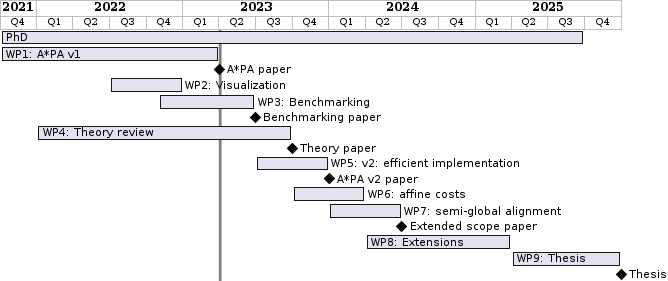
\includegraphics[width=.9\linewidth]{time-schedule.png}
\end{center}


\printbibliography

\newpage

\section{Teaching responsibilities}
\label{sec:orgd86de8d}
Teaching will take half a day to a full day a week. So far I have been a TA for
\emph{Datastructures for Population Scale Genomics} twice, and I plan to do this
again in upcoming fall semesters. I have made multiple (interactive)
\href{../alg-viz.org}{visualizations} (\href{../suffix-array-construction/suffix-array-construction.org}{suffix array construction}, \href{../bwt/bwt.org}{Burrows-Wheeler transform}) for this
course that can be reused in next years.
Currently I am helping with our groups seminar.

\section{Other duties}
\label{sec:org340ac7a}
Outside my PhD time, I am involved in the BAPC and NWERC programming contests as
a jury member.

\section{Study plan}
\label{sec:org07f3451}
I plan to take the following courses:

\begin{center}
\begin{tabular}{lrl}
Course & EC & Status\\\empty
\hline
Advanced Graph Algorithms and Optimization & 10 & Currently enrolled\\\empty
Poster presentation at IGGSY & 1 & Done\\\empty
Transferable skills course, likely Ethics, Science and Scientific Integrity & 1 & Later\\\empty
Academic paper writing & 2 & Optional\\\empty
\end{tabular}
\end{center}

\section*{Signatures}
\label{sec:org3db3f72}
\begin{itemize}
\item Supervisor, Prof. Dr. Gunnar  R\"{a}tsch:
        \vspace{4em}
\item Second advisor, Dr. Erik  Garrison:
        \vspace{4em}
\item Doctoral student, Ragnar Groot Koerkamp:

        \includegraphics[height=4em]{signature.jpg}
\item Date: March 2 2023
\end{itemize}
\end{document}
